% https://wiki.physik.uzh.ch/cms/latex:tikz:functions
    % Author: Izaak Neutelings (June, 2017)
% based on code from a friend

\documentclass{article}
\usepackage[top=0.25in]{geometry}
\usepackage{amsmath} % for \dfrac
\usepackage{tikz}
\tikzset{>=latex} % for LaTeX arrow head
\usepackage{pgfplots} % for the axis environment

%% split figures into pages
%\usepackage[active,tightpage]{preview}
%\PreviewEnvironment{tikzpicture}
%\setlength\PreviewBorder{1pt}%

\pagestyle{empty}

\begin{document}
	
	% DRAW PLOT: sin, cos, tan
	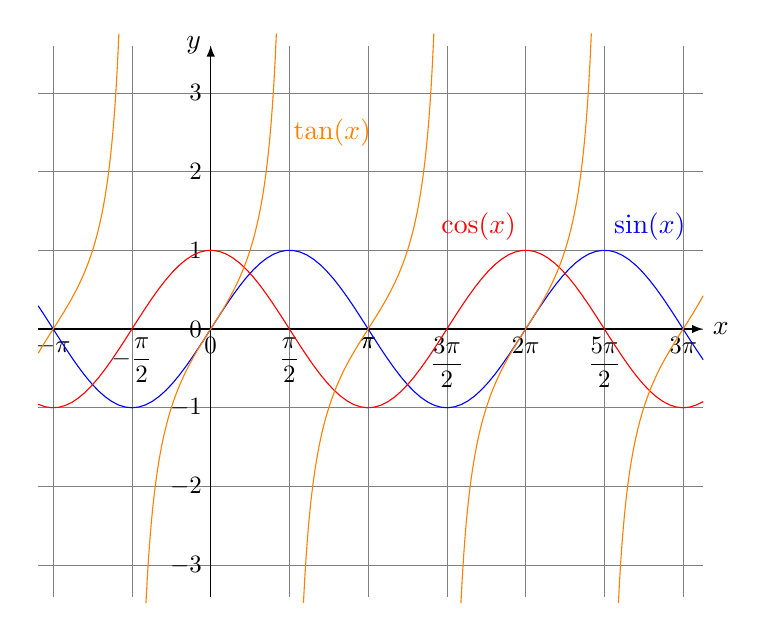
\begin{tikzpicture}[domain=-pi:pi,xscale=2/pi]
	
	% limits
	\def\xa{ -pi-0.3}
	\def\xb{3*pi+0.4}
	\def\ya{-3.4}
	\def\yb{ 3.6}
	\def\N{100} % number of points
	
	% axes & grid
	\draw[xstep=pi/2,very thin, color=gray]
	(\xa,\ya) grid (\xb,\yb);
	\draw[->]
	(\xa,0) -- (\xb,0)
	node[right] {$x$};
	\draw[->]
	(0,\ya) -- (0,\yb)
	node[left] {$y$};
	
	% ticks
	\draw[] % x
	node[below,scale=0.9] at ( -pi,   0) {$-\pi$}
	node[below,scale=0.9] at ( -pi/2, 0) {$-\dfrac{\pi}{2}$}
	node[below,scale=0.9] at (  pi,   0) {$\pi$}
	node[below,scale=0.9] at (     0, 0) {0}
	node[below,scale=0.9] at (  pi/2, 0) {$\dfrac{\pi}{2}$}
	node[below,scale=0.9] at (  pi,   0) {$\pi$}
	node[below,scale=0.9] at (3*pi/2, 0) {$\dfrac{3\pi}{2}$}
	node[below,scale=0.9] at (2*pi,   0) {$2\pi$}
	node[below,scale=0.9] at (5*pi/2, 0) {$\dfrac{5\pi}{2}$}
	node[below,scale=0.9] at (3*pi,   0) {$3\pi$};
	\draw[] % y
	node[left,scale=0.9] at ( 0,  3) {$3$}
	node[left,scale=0.9] at ( 0,  2) {$2$}
	node[left,scale=0.9] at ( 0,  1) {$1$}
	node[left,scale=0.9] at ( 0,  0) {$0$}
	node[left,scale=0.9] at ( 0, -1) {$-1$}
	node[left,scale=0.9] at ( 0, -2) {$-2$}
	node[left,scale=0.9] at ( 0, -3) {$-3$};
	
	% functions
	\def\ea{0.28}
	\def\eb{0.26}
	\draw[color=blue,samples=\N,domain=\xa:\xb] % SIN
	plot(\x,{sin(\x r)}) % r for radians
	node[above right] at (5*pi/2,1) {$\sin(x)$};
	\draw[color=red,samples=\N,domain=\xa:\xb] % COS
	plot(\x,{cos(\x r)})
	node[above left] at (2*pi,1) {$\cos(x)$};
	\draw[color=orange] % TAN
	plot[samples=\N,domain=  \xa     :   -pi/2-\eb] (\x, {tan(\x r)})
	plot[samples=\N,domain=  -pi/2+\ea:   pi/2-\eb] (\x, {tan(\x r)})
	plot[samples=\N,domain=   pi/2+\ea: 3*pi/2-\eb] (\x, {tan(\x r)})
	plot[samples=\N,domain= 3*pi/2+\ea: 5*pi/2-\eb] (\x, {tan(\x r)})
	plot[samples=\N,domain= 5*pi/2+\ea:  \xb      ] (\x, {tan(\x r)})
	node[samples=\N,right=-2pt] at (pi/2,2.5) {$\tan(x)$};
	
	\end{tikzpicture}
	
\vspace{24pt}
	
	% AXIS ENVIRONMENT: sin, cos, tan
	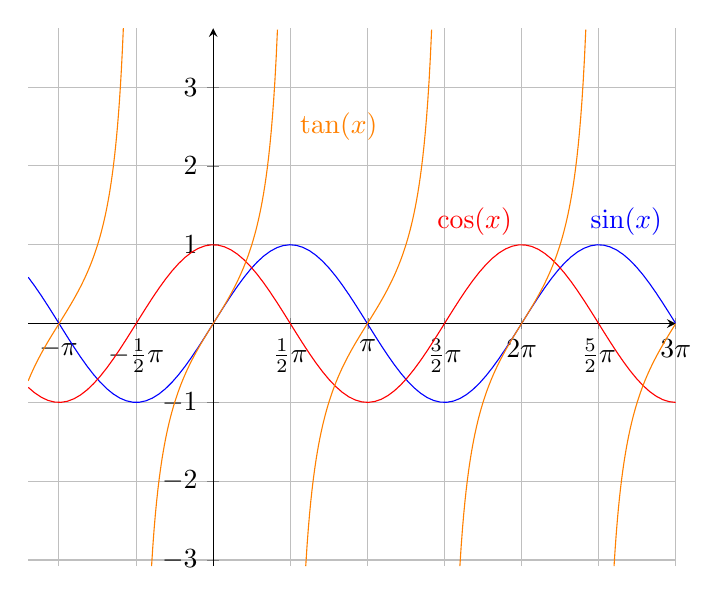
\begin{tikzpicture}
	\begin{axis}[enlargelimits=false,
	axis lines=middle,
	scale=1.2,
	xtick={-3.15159, -1.57080, 0,
		1.57080,  3.15159, 4.71239,
		6.28318,  7.85398, 9.42478 }, 
	xticklabels={$-\pi$, $-\frac{1}{2}\pi$, 0,
		$\frac{1}{2}\pi$, $\pi$, $\frac{3}{2}\pi$,
		$2\pi$, $\frac{5}{2}\pi$, $3\pi$ },
	ytick={-3,-2,-1,0,1,2,3},
	grid=major, % only a grid on the defined ticks
	samples=100 % number of points
	]
	
	% sin
	\addplot[blue,no marks,domain=-1.2*pi:3*pi]{sin(deg(x))}; % deg to convert radians
	\node[right=10pt,above] at (axis cs:5*pi/2,1){\color{blue}$\sin(x)$};
	
	% cos
	\addplot[red,no marks,domain=-1.2*pi:3*pi] {cos(deg(x))};
	\node[above left] at (axis cs:2*pi,1){\color{red}$\cos(x)$};
	
	% tan, multiple parts because of singularities
	\addplot[orange,no marks,domain=-1.2*pi:-0.583*pi, ]{tan(deg(x))};
	\addplot[orange,no marks,domain=-0.4*pi:5*pi/12,   ]{tan(deg(x))};
	\addplot[orange,no marks,domain=27*pi/45:17*pi/12, ]{tan(deg(x))};
	\addplot[orange,no marks,domain=1.6*pi:29*pi/12,   ]{tan(deg(x))};
	\addplot[orange,no marks,domain=2.6*pi:36*pi/12,   ]{tan(deg(x))};
	\node[right] at (axis cs:pi/2,2.5){\color{orange}$\tan(x)$};
	
	\end{axis}
	\end{tikzpicture}
	
\vspace{24pt}	
	
	% AXIS ENVIRONMENT: arcsin, arccos, arctan
	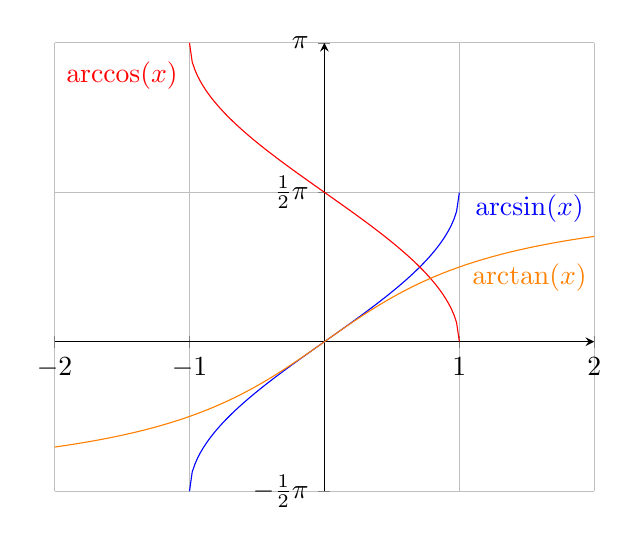
\begin{tikzpicture}
	\begin{axis}[enlargelimits=false,
	axis lines=middle,
	xtick={-2,-1,0,1,2},
	ytick={-1.570780, 1.570780, 3.14159},
	yticklabels={$-\frac{1}{2}\pi$,$\frac{1}{2}\pi$,$\pi$},
	grid=major,
	samples=100
	]
	
	% arcsin
	\addplot[domain=-1:1,no marks,blue] {rad(asin(x))};
	\node at (axis cs:1.52,1.4){\color{blue}$\arcsin(x)$};
	
	% arccos
	\addplot[domain=-1:1,no marks,red] {rad(acos(x))};
	\node at (axis cs:-1.5,2.8){\color{red}$\arccos(x)$};
	
	% arctan
	\addplot[domain=-2:2,no marks,orange] {rad(atan(x))};
	\node at (axis cs:1.52,.67){\color{orange}$\arctan(x)$};
	
	\end{axis}
	\end{tikzpicture}
	
\end{document}

